\chapter{Solución con sensores de fibra FBG\label{sec:FBG}}
%------------------------------
%------___SOLUCIÓN_FBG___------
%------------------------------

\label{sec:FBG3}

\textcolor{rositaoscuro}{
	\textit{
		\colorbox{yellow}{Introducción} breve del guante, que tecnologias implica.
		Resumen fibras de Bragg 
		¿Qué es una fibra FBG?
		¿Porque se utilizan?
		El procesado de las señales resultantes se realiza mediante Labview.
	}
}


 Como primer prototipo se ha estudiado y llevado a cabo un guante cuyo funcionamiento se basa en los sensores de fibra FBG. 
 
 El prototipo consiste en una sección de PDMS con forma de huella de mano que tiene embebida una red en fibra de Bragg. Para la obtención, procesado y visualización de los resultados medidos se emplea el entorno de desarrollo LabVIEW.


%--Marco conceptual
\section{Marco conceptual}
\label{sec:marco3}

Este apartado tiene por finalidad realizar una clara exposición de los conceptos teóricos fundamentales para la comprensión del diseño llevado a cabo. 


%--FIBRA ÓPTICA
\subsection{Fibra óptica}
\label{sec:fibra3}
	\textcolor{rositaoscuro}{
		\textit{
			- -Cómo se propaga la luz en ella.\\
	 		- -Partes de la fibra.\\
			Tipos de emisores (LED Laser).\\
			Receptores.\\
			Conectores y soldaduras.\\
			- -Fabricación.\\
			- -Tipos de fibra.\\
		}
	}

	%-- ¿Qué es la fibra óptica y la comunicación óptica?
	La fibra óptica es una hebra de material dieléctrico, así cómo el vidrio (sílice) o el polímero acrílico. 
	Se emplea como medio de propagación de señales luminosas. Es decir, para transmitir ondas electromagnéticas del espectro óptico: regiones espectrales de infrarrojo, luz visible y ultravioleta. En la siguiente imagen (figura \ref{fig:espectroOptico}) se puede observar dentro del espectro electromagnético dónde se sitúa el espectro óptico.	 
	
	\begin{figure}[H]
		\centering
		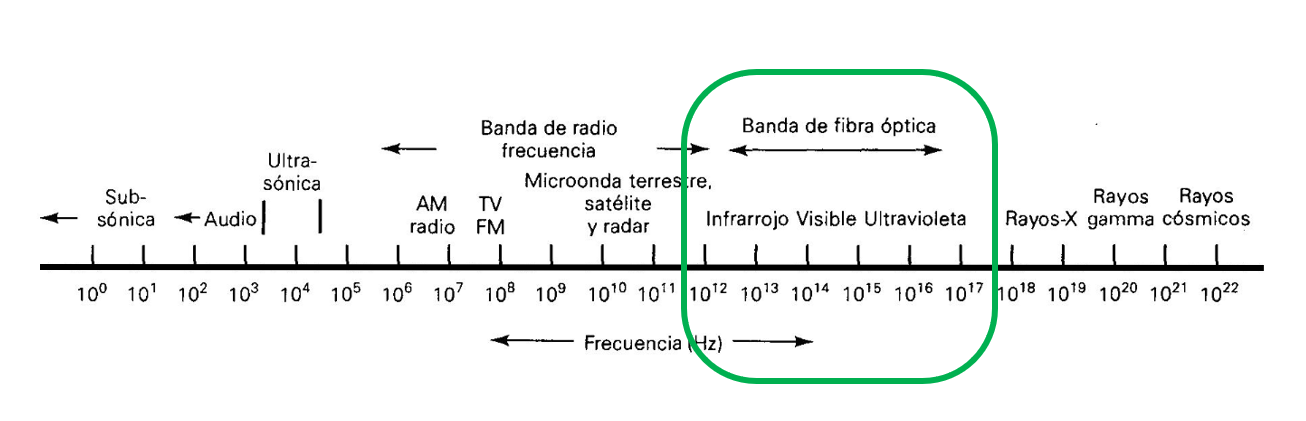
\includegraphics[width=0.95\textwidth]{./img/espectrooptico}
		\caption{Espectro electromagnético en frecuencia.}
		\label{fig:espectroOptico}
	\end{figure}
	
	%--Ventanas de comunicación por FO
	Cabe destacar que dentro del espectro óptico las longitudes de onda habituales para comunicación en fibra óptica están entre los 700nm y 1600nm. Estas se dividen en rangos con mejores características para la transmisión, denominadas ventanas de comunicación. Como se muestra en la figura \ref{fig:ventanaOptica}, son tres las ventanas más utilizadas,\cite{ventanasFO}:
 	\begin{table}[H]
		%\centering
		\hspace{2cm}
		\renewcommand{\arraystretch}{2}
		\begin{tabular}{rrl}
			\textbf{1ª ventana}& 800 a  900 nm  & $\longmapsto$ $\,$ longitud de onda utilizada = 850nm  \\
			\textbf{2ª ventana}& 1250 a 1350 nm & $\longmapsto$ $\,$ longitud de onda utilizada = 1310nm  \\
			\textbf{3ª ventana}& 1500 a 1600 nm & $\longmapsto$ $\,$ longitud de onda utilizada = 1550nm   \\ 
		\end{tabular} 
	\end{table}

	 \begin{figure}[H]
	 	\centering
	 	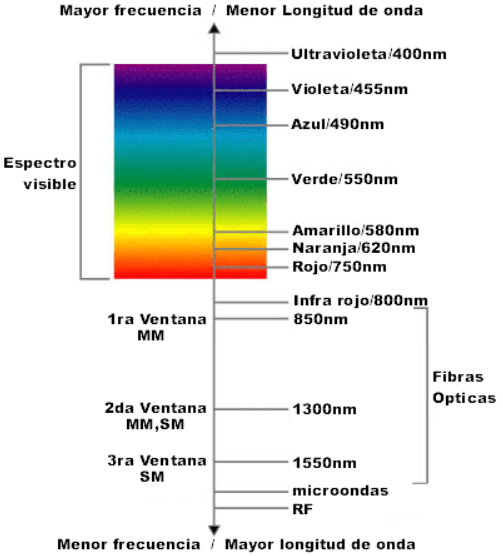
\includegraphics[width=0.5\textwidth]{./img/ventana}
	 	\caption{Longitud de onda fibra óptica junto con el espectro visible. \cite{ventanasFO}}
	 	\label{fig:ventanaOptica}
	 \end{figure}
 	La razón de que las ventanas de comunicación utilizadas se sitúen en las frecuencias indicadas reside en los diferentes comportamientos que tiene la atenuación de las señales en función de la longitud de onda (ver figura \ref{fig:perdidasFrec}). Existen algunas zonas dónde la atenuación es mínima, coincidiendo con la segunda y la tercera ventana. En cambio, en la zona correspondiente a la primera ventana las pérdidas no son mínimas, pero sí que se mantienen constantes. 	
 	
 	\begin{figure}[H]
 		\centering
 		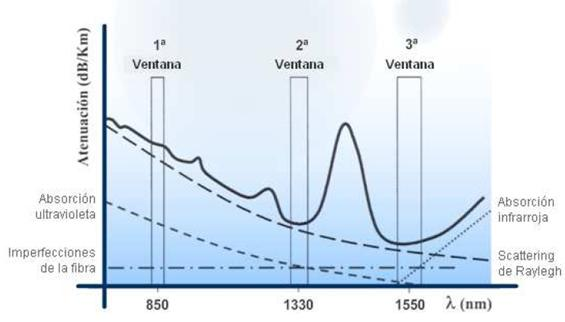
\includegraphics[width=0.8\textwidth]{./img/perdidasFrec}
 		\caption{Atenuación(dB/Km) frente a longitud de onda  $\lambda$ (nm) \cite{imgRadioModo}}
 		\label{fig:perdidasFrec}
 	\end{figure}

 %-- Características físicas de la fibra
 En cuanto a las propiedades físicas de la fibra óptica, son bastante delicadas ya que su grosor no supera por mucho al diámetro del cabello humano y se obtiene de la extrusión del sílice, SiO\textsubscript{2} , es decir, se trata de un filamento de vidrio muy fino. Es por ello que es la fibra óptica estándar está rodeada de una cubierta protectora. 
 
  \begin{figure}[H]
  	\centering
  	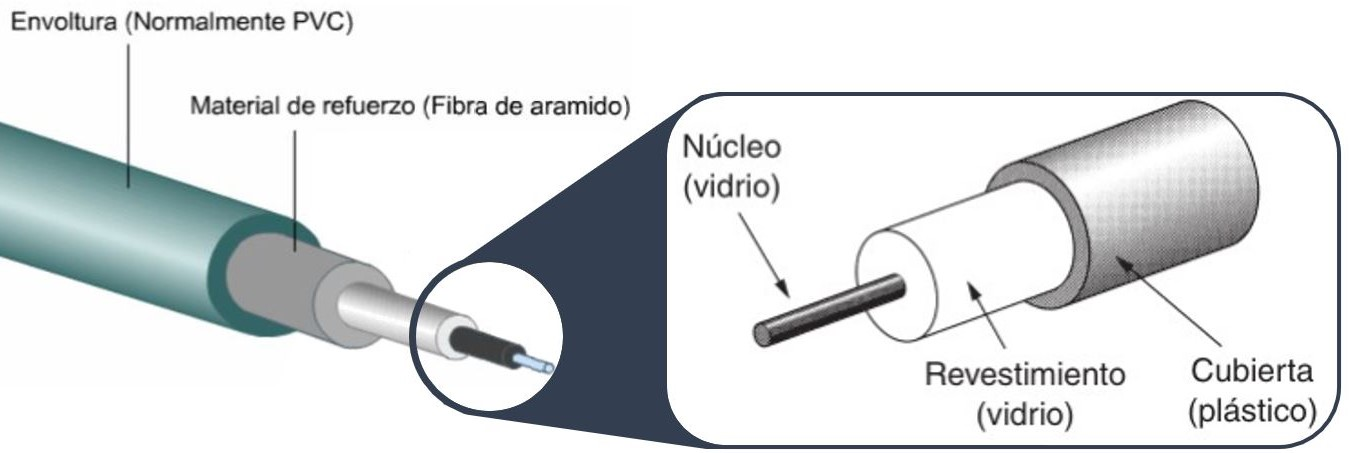
\includegraphics[width=0.87\textwidth]{./img/capas-fibra2}
  	\caption{Capas fibra óptica \cite{imgNucleoFibra,imgCapasFO}} 
  	\label{fig:capasFibra}
  \end{figure} 
  
  
  
 La fibra óptica estándar cuenta varias capas (figura \ref{fig:capasFibra}): núcleo, revestimiento y cubierta (o buffer).  Si la aplicación lo permite, conviene proteger la fibra con más capas externas. En la imagen anterior la fibra está además protegida por un material de refuerzo (fibra de aramido) y una envoltura (PVC).
 
 Tanto el núcleo cómo el revestimiento forman el medio por el cual se propaga la luz. Estas dos capas son tan finas que forman un filamento flexible, pero muy delicado, puesto que es muy propenso a romperse ante dobleces u otras manipulaciones externas. Por ello el resto de las capas son tambien importantes por proporcionar a la fibra protección y haciendo posible su utilización es escenarios de despliegue.
 
 %-- Fabricación FO
 La fabricación de la fibra óptica es un proceso de alta tecnología. Es importante mantener la pureza y la regularidad del núcleo. Esto es complejo, puesto que estamos hablando en algunos casos de núcleos de un grosor entorno a las 8 micras (en fibras monomodo). El grosor estándar de la fibra es de 125 micras(una micra equivale a una millonésima parte de un metro). Para conseguir este resultado el proceso de fabricación consiste en reproducir a escala macroscópica la estructura de la fibra que se quiere obtener. Esta reproducción a gran escala de la fibra deseada se le denomina preforma. Una vez se tiene la preforma, esta se va fundiendo y estirando hasta alcanzar el filamento del diámetro deseado. De una preforma se pueden sacar kilómetros de fibra. Para fabricar la preforma se parte de una barra de vidrio hueca (el vidrio que formará el recubrimiento) y se baña en un gas que contiene unas partículas (lo que formará el núcleo). Al calentar a mil grados, las partículas comienzan a fundirse hasta que el tubo colapsa y forma una vara maciza, que es la preforma. Para fundirla y estirarla esta se coloca verticalmente y se calienta. La complejidad de esta fase reside en mantener constante el flujo y el diámetro del hilo resultante. Además durante esta fase se aprovecha para crear una capa protectora sobre el vidrio (cubierta en la figura \ref{fig:capasFibra}). Finalmente los kilómetros de fibra óptica se enrollan en grandes bobinas. \cite{fabricacionFO}
 
 %-- Fibra Monomodo y multimodo
  \begin{figure}[H]
 	\centering
 	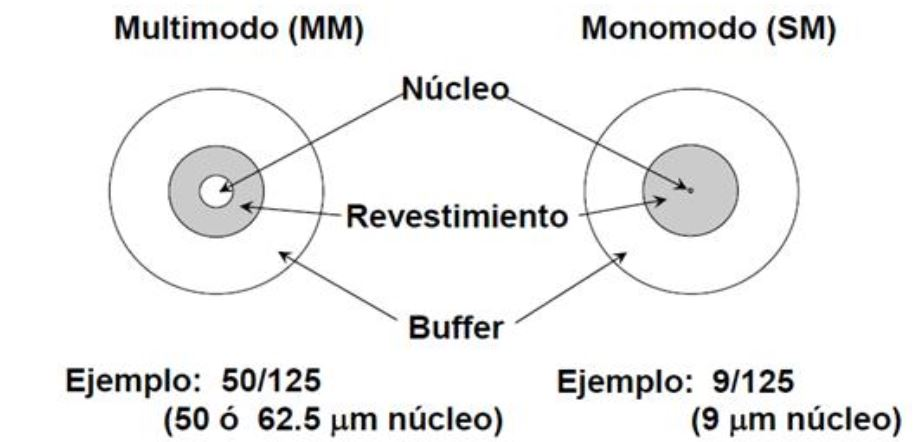
\includegraphics[width=0.6\textwidth]{./img/MM-SM}
 	\caption{Relación grosor fibra multimodo (MM) y monomodo (SM) \cite{imgRadioModo} } 
 	\label{fig:modoMonoMulti}
 \end{figure} 
 
  Dependiendo de la relación de diámetro entre el núcleo y el revestimiento, la fibra fibra será monomodo o multimodo (figura \ref{fig:modoMonoMulti}). Esta diferencia afecta a la propagación de la luz dentro de la guía de onda (figuras \ref{fig:guiaMM}, \ref{fig:guiaSM}, \ref{fig:indiceMultimodo}). Ya se ha comentado que el diámetro de la fibra es de aproximadamente 125 micras. En el caso de las fibras monomodo, el núcleo de estas tiene un diámetro tan pequeño (en torno a 8 micras) que la luz solo puede propagarse en un sólo modo (rayo). Sin embargo, en el caso de las fibras multimodo, al poseer un núcleo mayor (entre 50 o 62.5 micras) soportan la transmisión el múltiples modos, es decir, los rayos de luz viajan en muchas direcciones a través de este. \cite{FOA} 
   
   	\begin{figure}[H]
		\centering
		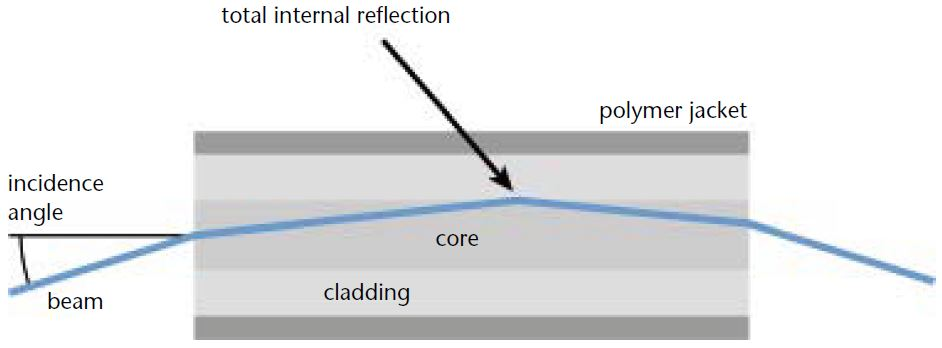
\includegraphics[width=0.7\textwidth]{./img/guiaMM}
		\caption{Corte transversal fibra multimodo en transmisión de luz. \cite{imgMonoMulti} } 
		\label{fig:guiaMM}
	\end{figure} 
  	\begin{figure}[H]
		\centering
		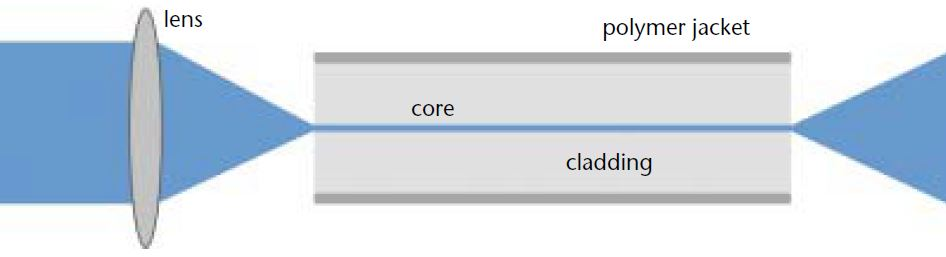
\includegraphics[width=0.7\textwidth]{./img/guiaSM}
		\caption{Corte transversal fibra monomodo en transmisión de luz. \cite{imgMonoMulti} } 
		\label{fig:guiaSM}
	\end{figure}  
 	
 	%-- Relación monomodo y multimodo con las longitudes de onda
 	Relacionando los tipos de fibras ópticas con las ventanas en las que trabajan, las fibras multimodo suelen trabajar en primera y segunda ventana, mientras que las fibras monomodo en segunda y tercera. 

	  	\begin{figure}[H]
		\centering
		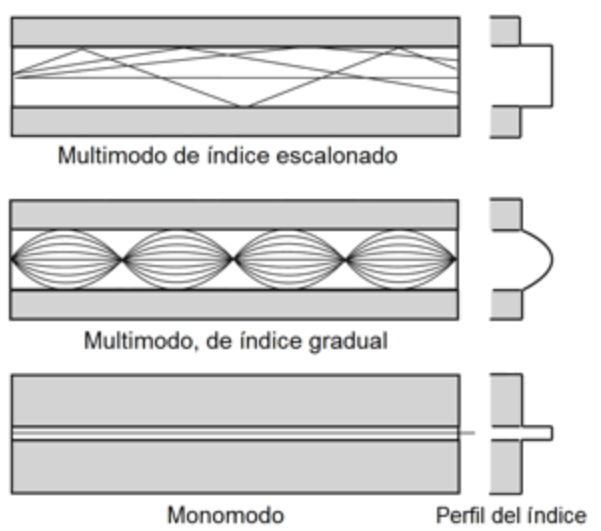
\includegraphics[width=0.5\textwidth]{./img/transFO-esc-grad}
		\caption{Disposición rayos. Multimodo (indice escalonado y gradual) y monomodo. \cite{FOA} } 
		\label{fig:indiceMultimodo}
		\end{figure}
	
 	%-- Otros tipos de FO
 	Además existen otros tipos de fibras menos comunes: la fibra de plástico (POF) y la fibra de sílice con revestimiento de plástico (HCS/PCS). La primera tiene un núcleo de gran diámetro ($1mm$ aproximadamente), puede utilizarse para redes de distancia corta y de baja velocidad. Las fibras de sílice con revestimiento de plástico tienen un núcleo más pequeño ($200\mu m$ aproximadamente) que las fibras de plástico. Estos dos últimos tipos de fibra multimodo generalmente son de índice escalonado, mientras que el resto de fibras multimodo suelen ser de índice gradual. En la figura \ref{fig:indiceMultimodo} se observa como es la diferencia en la distribución de los rayos en un caso y en el otro. En cuanto al tamaño de las fibras, la figura \ref{fig:otrosTiposFO} se representan las diferentes relaciones de tamaños entre los cinco tipos de fibra vistos. \cite{FOA}
 	 	
 	 \begin{figure}[H]
 	 	\centering
 	 	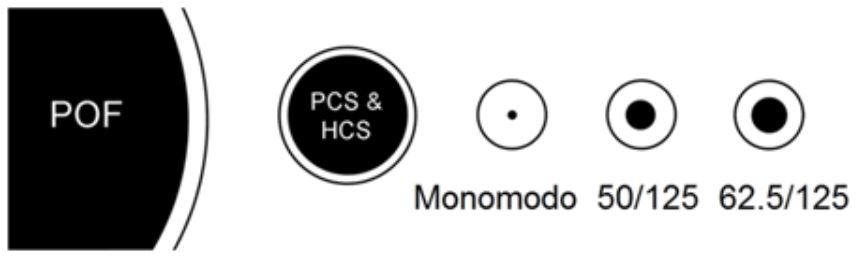
\includegraphics[width=0.7\textwidth]{./img/tiposFO}
 	 	\caption{Relación tamaños fibras ópticas. \cite{FOA} } 
 	 	\label{fig:otrosTiposFO}
 	 \end{figure} 	
  	
 %-- PROPAGACIÓN DE LA LUZ	
 %-- Diferenci de indices de refracción
 La diferencia de índices de refracción entre las capas centrales de la fibra son las que permiten la propagación de la luz a través de esta. El núcleo tiene un mayor indice de refracción que el revestimiento, lo que genera que los rayos de luz se curven a medida que pasan del núcleo al revestimiento, generando una "reflexión interna total" en la fibra. La siguiente imagen (figura \ref{fig:TIR}) sirve para explicar claramente este concepto:
 
 \begin{figure}[H]
 	\centering
 	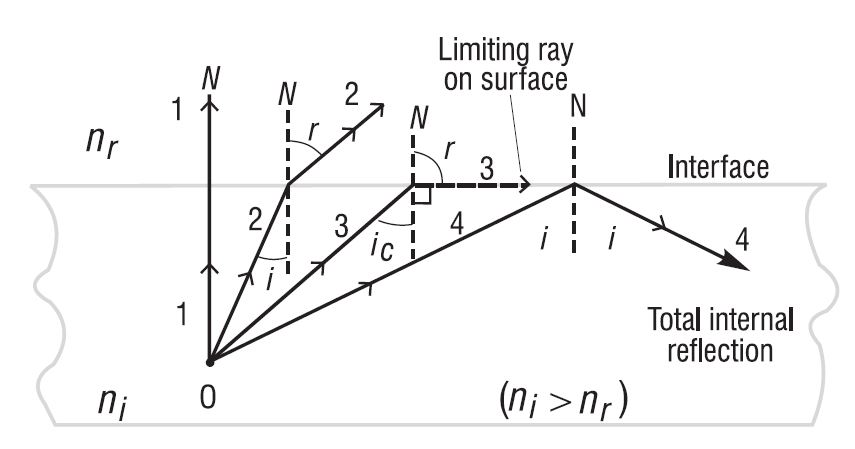
\includegraphics[width=0.66\textwidth]{./img/TIR}
 	\caption{Ángulo crítico y reflexión interna total. \cite{geometriaBasicaFP} } 
 	\label{fig:TIR}
 \end{figure}
 
 %Reflexión interna total
 En la figura \ref{fig:TIR} se ilustran cuatro rayos que se originan en el puno 0, lo que sería el núcleo de la fibra óptica (dónde el indice de refracción \textit{n\textsubscript{i}} es mayor). Entre los cuatro rayos varía el ángulo con el que estos inciden sobre el revestimiento (de menor índice de refracción\textit{n\textsubscript{r}}). Se observa cómo en el rayo número 1 incide con $90\,^{\circ}$ (incidencia normal), no habiendo reflexión y siguiendo el rayo en la misma dirección. En el rayo número 2 incide con un ángulo \textit{i}, y se refracta con \textit{r}. El rayo número 3 incide con el ángulo crítico \textit{i\textsubscript{c}}, suficientemente grande para que el rayo reflejado se propague a lo largo de la interfaz entre los dos medios, quedando atrapado. Por último, el rayo número 4 incide con un ángulo \textit{i} superior al ángulo crítico (ecuación \ref{eq:angCritico}), \textit{i\textsubscript{c}}, consiguiendo que se refleje totalmente en el mismo medio del que incide. Este rayo obedece a la ley de reflexión, siendo su ángulo de reflexión exactamente igual a su ángulo de incidencia. Este fenómeno se denomina \textit{"Reflexión interna total"}, necesario para que suceda la transmisión de señales lumínicas en la fibra óptica. 

	\begin{equation}
		\label{eq:angCritico}
		\hat{i}\textsubscript{c} =  \sin^{-1}\left(\dfrac{n\textsubscript{r}}{n\textsubscript{i}}\right)
	\end{equation}

 La reflexión interna total atrapa la luz hasta cierto ángulo en el núcleo, definiendo la apertura numérica a la que hay que asegurarse de penetrar la luz para que se de el fenómeno de reflexión interna total. Así se fuerza a que la mayoría de los rayos de luz incidan sobre el interfaz y se reflejen, permitiendo la transmisión de la señal lumínica. 
 
 
 \textcolor{rositaoscuro}{//----------------------------------------------------------------------- }\\ 
 %No vamos a hablar más de multimodo
 \textcolor{teal}{(\\Puesto que en la solución llevada a cabo en este trabajo se utilizan fibras monomodo no se va a extender el texto en explicar más conceptos sobre la transmisión en fibras multimodo.\\)\\
 \textcolor{rositaoscuro}{-------------------------------------------------------------------------//}\\}
 
 
 %Sistemas de propagación
   \begin{figure}[H]
 	\centering
 	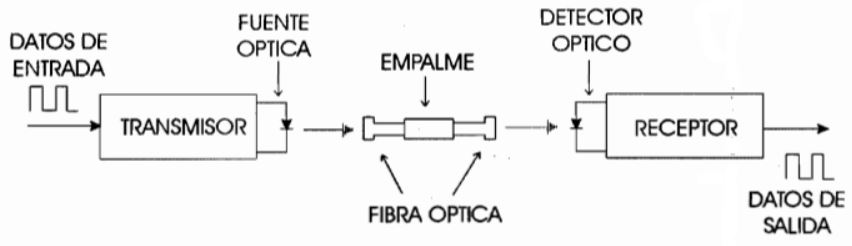
\includegraphics[width=1\textwidth]{./img/TxFOp2p}
 	\caption{Transmisión punto a punto de señales a través de fibra óptica. \cite{txFO} } 
 	\label{fig:TxFOp2p}
 \end{figure} 
 
 Los sistemas de propagación de señales luminosas a través de la fibra óptica componen un medio de transmisión de datos rápido y fiable. En la figura \ref{fig:TxFOp2p} se plasma el procedimiento que sigue la transmisión de datos en un sistema óptico y los elementos que lo componen. Previa a la propagación a través de un medio óptico de una señal eléctrica (analógica o digital) es necesario realizar una conversión de esta a señal óptica. Esto genera una señal óptica a partir de una señal eléctrica en el emisor o fuente de luz situado en el extremo inicial de la comunicación. Realizada la conversión, la señal es transmitida a lo largo de la fibra óptica. Según las características del escenario puede haber una o varias uniones entre fibras a lo largo del canal. Estás pueden realizarse empalmando o utilizando conectores. Una vez la señal óptica atraviesa todo el canal, llega al detector, dónde sucede el proceso inverso al ocurrido en el emisor y a la salida del sistema completo se tiene la señal eléctrica. Esta corresponde a la señal introducida al sistema con una pequeña posibilidad de haber sufrido pérdidas o atenuación debido a la impureza de la fibra, la distancia, las conexiones entre elementos del sistema o cualquier otro evento ajeno al este. Estas modificaciones de la señal de entrada pueden ser contrarrestadas o solventadas en recepción sin suponer un impedimento a una comunicación exitosa.    
  
 Veamos por separado los elementos dibujados en la figura \ref{fig:TxFOp2p}:
 	\begin{itemize}
 	%-Emisores (Transmisión)
 		\item \textit{\textbf{Emisores (Transmisión)}}	
 		% \hspace{0.2cm} 
 		Los emisores de luz forman un papel imprescindible en la transmisión de señales a través de la fibra óptica. Se encargan de convertir la señal eléctrica a señal luminosa, para que esta se pueda propagar por el canal óptico según lo esperado. Principalmente hay dos tipos de fuentes de luz: diodos LED o diodos láser. Dentro de los de tipo láser se distinguen otros tres tipos: láser fabry-perot (\textit{FP}), láser de retroalimentación distribuida (\textit{(DFB)}) y láser de cavidad vertical y emisión superficial (\textit{VCSEL}). Unas de las condiciones más importantes que deben cumplir las fuentes de luz son que operen en la longitud de onda adecuada, se puedan de modular lo suficientemente rápido para transmitir datos y poder acoplarse de forma eficiente a la fibra. \cite{TransRecepFO}
 		
 		 \begin{figure}[H]
 			\centering
 			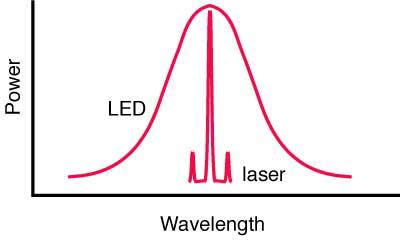
\includegraphics[width=0.35\textwidth]{./img/led-laser}
 			\caption{Relación entre potencia y longitud de onda diodo LED frente a diodo láser. \cite{FOA} } 
 			\label{fig:ledVsLaser}
 		\end{figure} 
 	 	\begin{figure}[H]
 			\centering
 			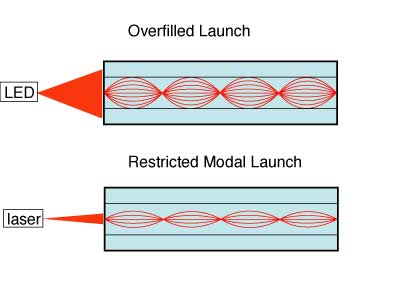
\includegraphics[width=0.55\textwidth]{./img/led-laserEMISION}
 			\caption{Corte transversal de fibra con emisión desde diodo LED frente a diodo láser. \cite{FOA} } 
 			\label{fig:corteledVsLaser}
 		\end{figure} 
 		
 		\begin{itemize}
 			\item \textbf{LED} - \textit{Light Emitting Diodes}\\
 			Consiste en una fuente de luz incoherente. Es una fuente de luz de mayor ancho de banda de operación que en el caso de los diodos láser (véase figura \ref{fig:ledVsLaser} y \ref{fig:corteledVsLaser}). Tiene un espectro de emisión entre los 30-100 nm. En función del material semiconductor con el que se fabrique se pueden emitir desde luz ultravioleta hasta infrarrojos. Para conseguir emitir en un espectro reducido, es necesario polarizarlo y hacerle circular corriente eléctrica. Pueden ser modulados sin dificultad hasta velocidades de 100-200 Mb/s y en algunos casos hasta velocidades de 1 Gb/s. 
 			
 			Además, tienen un comportamiento simple, de fácil fabricación y tienen un coste bajo en comparación a otras fuentes. Su circuitería de alimentación y control es muy sencilla, debido a los bajos niveles de corriente que son necesarios para que funcione el dispositivo y a su relativa inmunidad frente a variaciones de la temperatura. Necesitan baja potencia de alimentación. Su geometría y patrón de radiación es de alta divergencia, el acoplo de luz a la fibra óptica monomodo es difícil, especialmente en los LED de emisión superficial. Son dispositivos fiables, ya que no sufren la degradación de tipo catastrófico y son menos sensibles que los diodos láser a la degradación por envejecimiento. \\
 			
 					\textcolor{rositaoscuro}{//-Resumen: Los LED se basan en emisión espontánea. Por sus características (baja coherencia, divergencia alta, baja potencia óptica de salida, circuitos electrónicos sencillos,...) se emplean habitualmente en combinación con fibras multimodo para enlaces de distancias cortas y velocidades bajas.}
 			
 			\item \textbf{Láser} - \textit{Light Amplification by Stimulated Emission of Radiation}\\
 			Consiste en un tipo de fuente de luz coherente. Tienen mayor capacidad de transmisión de luz, concentran la luz en forma de haces estrechos pero potentes, es decir, emiten de manera direccional e intensa. Es por ello que se suele advertir que mirar con los ojos directamente a este tipo de emisiones es peligroso para la vista. (Véanse figuras \ref{fig:ledVsLaser} y \ref{fig:corteledVsLaser}). Pueden ser modulados en frecuencia y a gran velocidad. Su geometría y patrón de radiación es de relativamente baja divergencia, el acoplo de luz a la fibra óptica monomodo es bastante eficiente. Su composición es más compleja que la del diodo LED. Para conseguir dicha directividad y potencia, internamente la fuente tiene cavidades que combinan medio activo y espejos. Por ejemplo, necesita tener un circuito de realimentación para su control, debido a que se ve afectado por las variaciones de temperaturay a las reflexiones que pueda provocar la potencia óptica incidente en su salida. Debido a ello, son complejos y costosos de fabricar. 
 			
 					\textcolor{rositaoscuro}{//- Resumen Los láseres se basan en emisión estimulada, conseguida formando cavidades que combinan medio activo y espejos para la realimentación. Son de mayores prestaciones que los LED (mayor coherencia, más directivos, mayor potencia de salida,...), pero más complejos y caros. Se pueden usar en fibras monomodo. Los hay de dos tipos, básicamente:\\
 					--Láseres multimodo (Fabry-Perot) que se usan en enlaces de velocidades medias/bajas para distancias medias/cortas\\
 					-- Láseres monomodo (DFB,DBR) que se usan en enlaces de alta capacidad –alta velocidad, distancias largas- y en sistemas WDM}
 			
 			
 		\end{itemize}
  		
  		La tabla \ref{tabla:caractFuentes} compara las características de las diferentes fuentes mencionadas, permitiendo ver también las diferencias entre los diferentes tipos de diodos láser citados.
  		
  		
  		\begin{table}[H]
  			\begin{tabular}{l|c|c|c|c|}
  				\cline{2-5}
  				& \cellcolor[HTML]{EFEFEF}\textbf{LED} & \cellcolor[HTML]{EFEFEF}\textbf{LD F-P} & \cellcolor[HTML]{EFEFEF}\textbf{LD\_DFB} & \cellcolor[HTML]{EFEFEF}\textbf{VCSEL} \\ \hline
  				\multicolumn{1}{|l|}{\cellcolor[HTML]{EFEFEF}Espectro emisión}                 & Ancho                                & Medio                                   & \multicolumn{2}{c|}{Estrecho}                                                     \\ \hline
  				\multicolumn{1}{|l|}{\cellcolor[HTML]{EFEFEF}Directividad}                     & Muy divergente                       & \multicolumn{3}{c|}{Directivo}                                                                                              \\ \hline
  				\multicolumn{1}{|l|}{\cellcolor[HTML]{EFEFEF}Potencia}                         & Baja                                 & \multicolumn{3}{c|}{Alta}                                                                                                   \\ \hline
  				\multicolumn{1}{|l|}{\cellcolor[HTML]{EFEFEF}Velocidad / BW modulación}        & Varios cientos de MHz                & \multicolumn{3}{c|}{Varias decenas de GHz}                                                                                  \\ \hline
  				\multicolumn{1}{|l|}{\cellcolor[HTML]{EFEFEF}Acoplo a la fibra}                & MMF                                  & \multicolumn{2}{c|}{SMF}                                                           & MMF                                    \\ \hline
  				\multicolumn{1}{|l|}{\cellcolor[HTML]{EFEFEF}Curva I-P}                        & Sin $I_{umbral}$; baja pendiente          & \multicolumn{3}{c|}{Con $I_{umbral}$; alta pendiente}                                                                            \\ \hline
  				\multicolumn{1}{|l|}{\cellcolor[HTML]{EFEFEF}Dependencia con temperatura}      & Baja                                 & \multicolumn{3}{c|}{Alta}                                                                                                   \\ \hline
  				\multicolumn{1}{|l|}{\cellcolor[HTML]{EFEFEF}Circuitos electrónicos asociados} & Sencillos                            & \multicolumn{3}{c|}{Complejos}                                                                                              \\ \hline
  				\multicolumn{1}{|l|}{\cellcolor[HTML]{EFEFEF}Seguridad para la vista}          & No peligroso                         & \multicolumn{3}{c|}{Potencialmente dañino}                                                                                  \\ \hline
  				\multicolumn{1}{|l|}{\cellcolor[HTML]{EFEFEF}Tiempo vida útil}                 & Alto                                 & \multicolumn{3}{c|}{Medio (suficiente)}                                                                                     \\ \hline
  				\multicolumn{1}{|l|}{\cellcolor[HTML]{EFEFEF}Coste}                            & Bajo                                 & Medio                                   & Alto                                     & Bajo                                   \\ \hline
  				\multicolumn{1}{|l|}{\cellcolor[HTML]{EFEFEF}Ventana operación}                & 1ª, 2ª                               & \multicolumn{2}{c|}{2ª, 3ª}                                                        & 1ª, 2ª                                 \\ \hline
  			\end{tabular}
  		\caption{Tabla características fuentes de ópticas}
  		\label{tabla:caractFuentes}
  		\end{table}
  	
   	%-Detectores (Recepción)		
 		\item \textit{\textbf{Detectores (Recepción)}}
 			
 		En cuanto al proceso de recepción, consiste en que la señal llega al final del canal y se tiene que dar el proceso inverso que en transmisión. Los detectores tienen la función de convertir las señales ópticas a señales eléctricas para recuperar la información. Son diodos semiconductores encargados de polarizar inversamente la polarización realizada en el diodo emisor.  Al igual que pasaba en la transmisión, existe detección coherente o incoherente(detección directa). El componente del receptor que realiza la conversión óptico-eléctrica es el fotodetector. Se distinguen varios tipos, los más comunes son: los fotodidos PIN y los fotodiodos de efecto de avalancha (\textit{APD}). Aunque merece la pena mencionar los fotoespectrómetros, formados por células CCD integradas y una estructurá optica tan precisa que es capaz de detectar la potencia que la luz recibida proporciona en cada longitud de onda. Volviendo a los receptores PIN y APD, además del fotodetector, el detector puede estar compuesto por un pre-amplificador óptico, pero casi siempre tendrá un pre-amplificador eléctrico para amplificar la señal eléctrica obtenida del fotodiodo, de muy baja corriente. El receptor lo podrá formar también (figura \ref{fig:diagRX}) un filtro óptico, para tomar solo en cuenta las frecuencias de interés. Posterior a la pre-amplificación eléctrica, los elementos de procesado de la señal que se incluyan dependerán del si las señales empleadas por el sistema eléctrico son analógicas o digitales.
 		
	 	\begin{figure}[H]
	 		\centering
	 		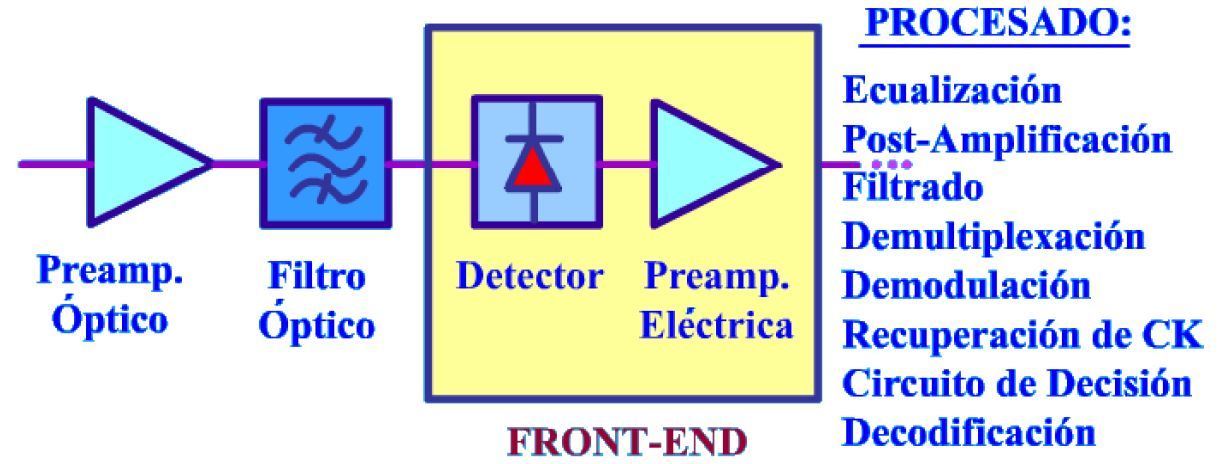
\includegraphics[width=0.65\textwidth]{./img/diagRX}
	 		\caption{Diagrama de bloque receptor} 
	 		\label{fig:diagRX}
	 	\end{figure} 
 	
 		Idealmente los fotodetectores deberián ser altamente sensibles, con alta velocidad de respuesta, poco ruidosos, compactos, robustos y de respuesta lineal. En la práctica es complicado conseguir todos estos atributos en conjunto. Por ejemplo, los APD requieren menor potencia óptica para funcionar que los diodos PIN, pero cuatro veces mayor voltaje de alimentación.
 		
 		\textcolor{rositaoscuro}{//---------------------------------------------------Puedo añadir si eso lo que pone en el siguiente link:}
 		\url{http://www.thefoa.org/tech/ref/appln/transceiver.html}
 	
 	%-Conectores y empalmes
 		\item \textit{\textbf{Conectores y empalmes}}\\

 		Cabe hablar también de los conectores ópticos y empalmes utilizados para unir fibra óptica a fibra óptica u otros elementos del sistema. Teniendo una fibra óptica terminada en algún tipo de conector esta se puede unir a elementos como emisores, receptores, multiplexores y otros elementos, incluso se puede unir a otra fibra terminada en conector con un adaptador macho a macho. Además, para unir dos trozos de fibra es posible realizar una fusión que empalme ambas terminaciones de la fibra. La principal diferencia entre estos dos tipos de uniones es que los conectores unen de manera no permanente, mientras que los empalmes son uniones permanentes. 
 		
 		\begin{figure}[H]
 			\centering
 			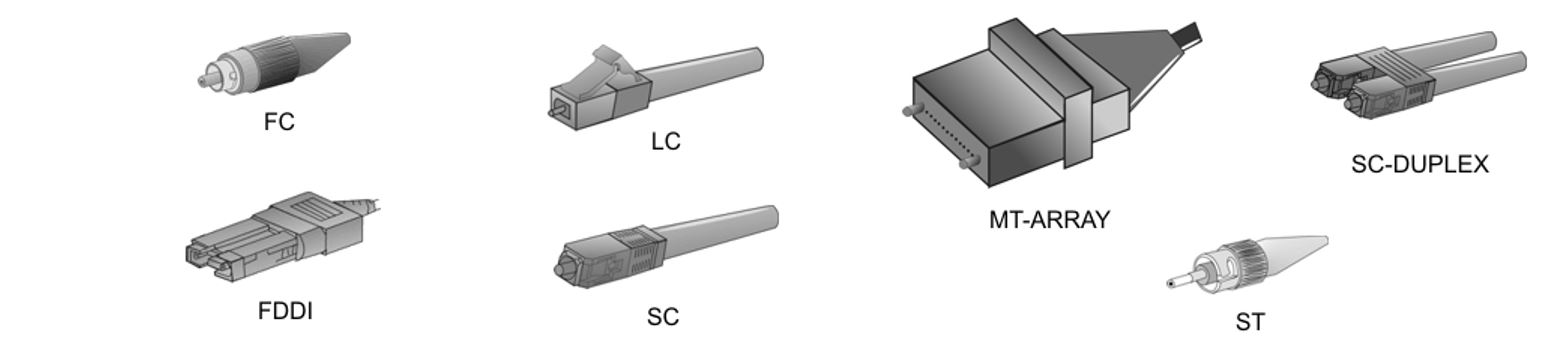
\includegraphics[width=0.95\textwidth]{./img/tiposConect2}
 			\caption{Tipos de conectores de fibra óptica. \cite{TipConectoresFO}} 
 			\label{fig:tiposConect}
 		\end{figure} 
 		
 		Es importante que las uniones no afecten a la calidad de la transmisión, es decir, deben garantizar bajas pérdidas de conectividad. En la figura \ref{fig:tiposConect} se muestra algunos de los conectores más empleados, cada uno de ellos suelen utilizarse en diferentes aplicaciones según sus características. Por ejemplo los utilizados en este trabajo, los conectores FC (\textit{Ferule Connector}) se suelen utiliza tanto en montaje de laboratorio como de campo y sirven en fibras monomodo y multimodo. Además tienen unas pérdidas de inserción IL < 0.34 dB en fibras multimodo y IL < 0.15 dB en fibras monomodo. \cite{TipConectoresFO}\\
 		\begin{figure}[H]
	 		\centering
	 		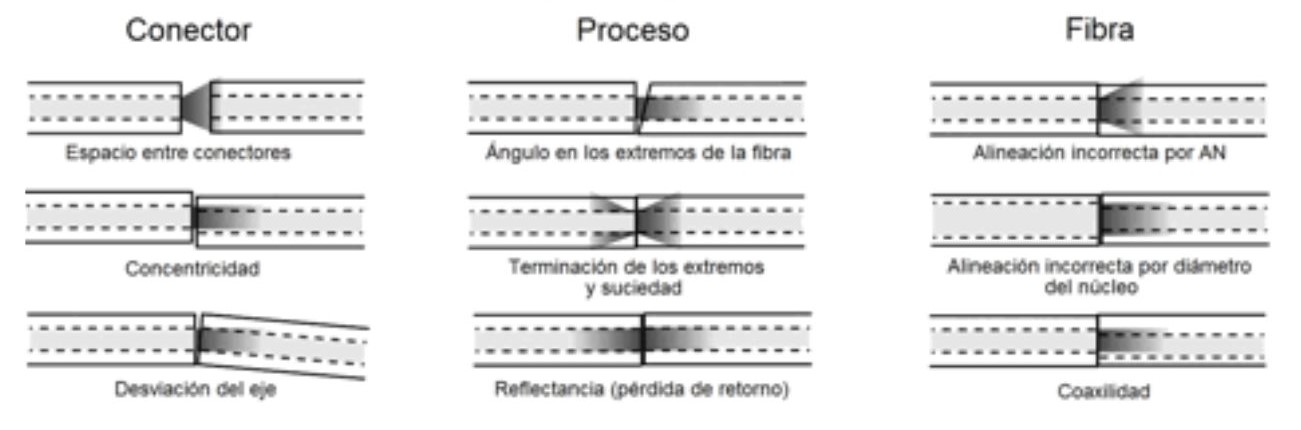
\includegraphics[width=0.85\textwidth]{./img/perdidasOpticas}
	 		\caption{Causas de pérdida óptica en las uniones. \cite{FOAconect}} 
	 		\label{fig:conectLoss}
 		\end{figure}
 		Las pérdidas se pueden reducir cuando los núcleos de las dos fibras son idénticos, están alineados de manera perfecta y se tocan entre sí, los conectores y los empalmes se realizaron adecuadamente y no hay suciedad en la unión. En la figura \ref{fig:conectLoss} se pueden observar diferentes causas de pérdidas en las conexiones de fibra óptica. Además, los conectores pueden tener diferentes formas de férulas (o terminaciones), diferentes tipos de pulidos en el extremo de la fibra donde se realiza la unión (figura \ref{fig:tiposPulidos}), lo que afecta también a las pérdidas resultantes. El extermo de la fibra tiene que estar debidamente limpio y pulido para reducir al máximo ñas pérdidas, ya que una superficie aspera puede dispersar o absorber luz.		
   		\begin{figure}[H]
   			\centering
   			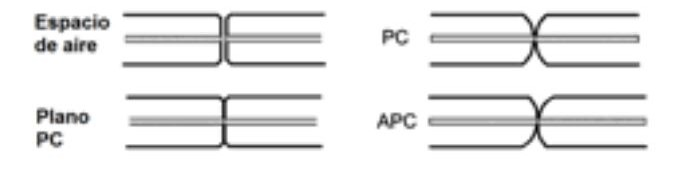
\includegraphics[width=0.55\textwidth]{./img/conectoresPulido}
   			\caption{Tipos de conectores según su pulido. \cite{TipConectoresFO}} 
   			\label{fig:tiposPulidos}
   		\end{figure}

 		En cuanto a los empalmes, que crean una unión permanente entre dos fibras, hay dos tipos: por fusión y mecánicos. En la figura \ref{fig:empalmeTipo} se observa en primer lugar un empalme por fusión y los demás son mecánicos. Los más realizados son los empalmes por fusión por la fiabilidad y la robustez de la unión, así como por brindar pérdidas y reflectancias menores.
 		
 		\begin{figure}[H]
 			\centering
 			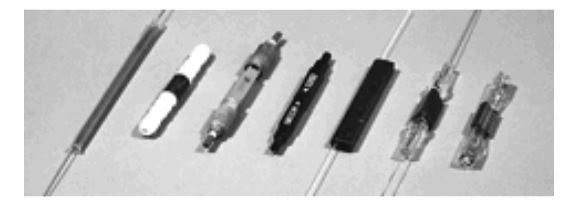
\includegraphics[width=0.5\textwidth]{./img/tiposEmpalme}
 			\caption{Tipos de empalmes. \cite{FOAconect}} 
 			\label{fig:empalmeTipo}
 		\end{figure} 
 	
 		 
 		
 		El proceso de fusión (Figura \ref{fig:procFusion}) consiste en primero pelar, limpiar y cortar los extremos de las fibras que se desee unir. Una vez se dispone en los extremos de la fibra desnuda, cortada con la cortadora de precisión y limpia con un paño adecuado y alcohol, se deben colocar cada una en las guías de la fusionadora. Después se ejecuta el programa de fusión adecuado, según sea la fibra. Por último, se le coloca a la fusión un manguito protector termocontraible o una protección tipo mordaza para que la fusión no se desprenda ante alguna adversidad.
 		
 		\begin{figure}[H]
 			\centering
 			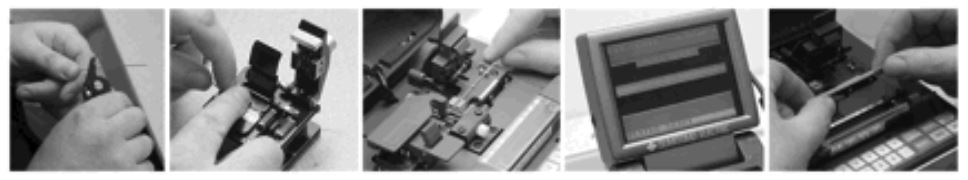
\includegraphics[width=0.85\textwidth]{./img/procesoFusion}
 			\caption{Proceso de empalme por fusión. \cite{FOAconect}} 
 			\label{fig:procFusion}
 		\end{figure}

 	 \end{itemize}					

%-- SENSORES ÓPTICOS	
\subsection{Sensores ópticos} %Tipos de sensores ópticos
\label{sec:sensores3}

		
		Existen en el mercado diversos tipos de sensores ópticos. Estos se pueden clasificar atendiendo a diversos aspectos. A continuación se exponen dos clasificaciones básicas\cite{sensoresOpticos}: 

			\begin{itemize}
				\item[$\cdot$] \underline{En función de la naturaleza del parámetro a cuantificar}
				\begin{itemize}
					\item Sensores químicos: Sirven para detectar variación de cantidad de ciertos componentes químicos. Además en este grupo se incluyen los biosensores.
					\item Sensores físicos: Utilizados para medir parámetros físicos (temperatura, presión, espesor, etc.)
				\end{itemize}
				\item[$\cdot$] \underline{En función de la naturaleza de la propiedad óptica medida}
				\begin{itemize}
					\item Sensores de absorbancia
					\item Sensores de reflectancia
					\item Sensores se luminiscencia (fluorescencia, quimioluminiscencia y bioluminiscencia)
					\item Sensores de dispersión Raman
					\item Sensores de índice de refracción
					\item etc.
				\end{itemize}
				\end{itemize}
			
			
				En este trabajo se van a utilizar sensores de difracción de Bragg, que son sensores que cuantifican parámetros físicos a través de mediciones ópticas del índice de refracción.
		
	\begin{itemize}
		\item \textit{\textbf{Redes de difracción de Bragg \textit{(FBG - Fiber Bragg Grating)}}}	
		
		\begin{figure}[H]
			\centering
			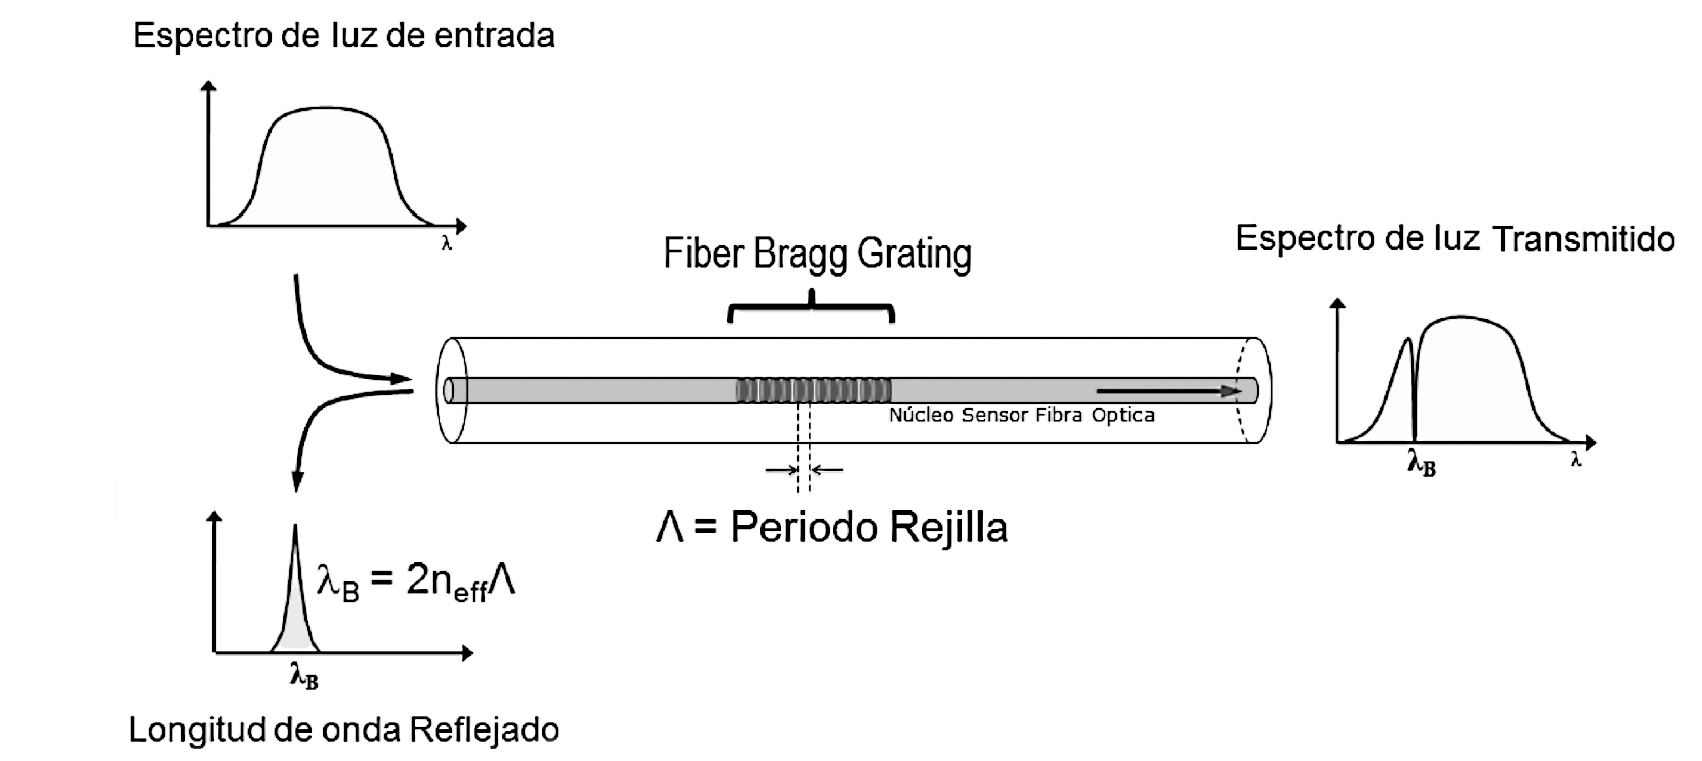
\includegraphics[width=0.85\textwidth]{./img/operacionFBG}
			\caption{Funcionamiento de un sensor de fibra óptica FBG \cite{funcionamientoFBG}} 
			\label{fig:funcionamientoFBG}
		\end{figure}		
		
		Los sensores de fibra óptica basados en redes de difracción de Bragg (\textit{Fibre Brag Gratings}), también denominadas FBGs, están diseñados para reflejar longitudes de onda determinadas (según el diseño) de la luz y transmitir el resto (Figura \ref{fig:funcionamientoFBG}). Para ello se crea en el núcleo de la fibra una variación periódica del índice de refracción, conocido cómo rejilla tipo Bragg. Esta variación sólo afecta a la transmisión de cierta longitud de onda, la que refleja. Este tipo de fenómeno se puede utilizar cómo filtro bloqueador de una longitud de onda, además de para medir parámetros físicos cómo la deformación o la temperatura. Por ejemplo, es muy común su uso para la monitorización de estructuras como puentes \cite{FOSensorFrancis}. 
		
		\begin{figure}[H]
			\centering
			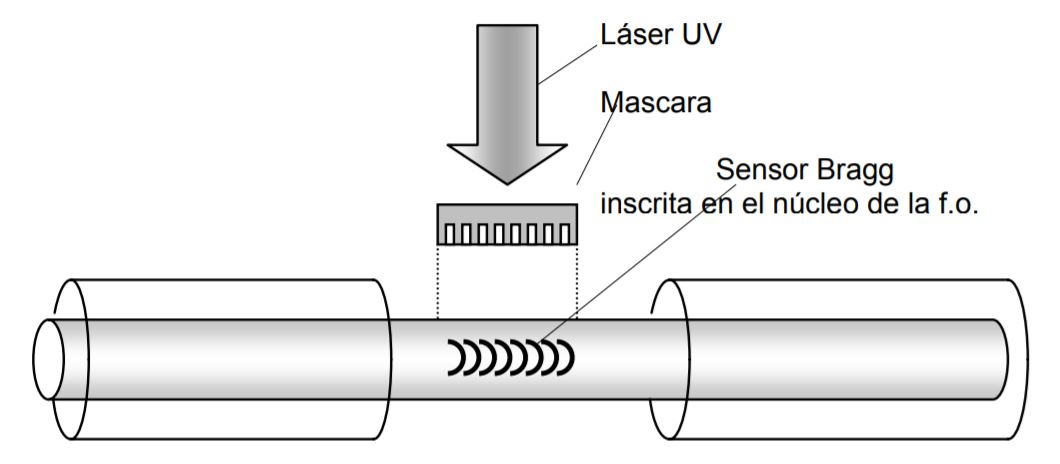
\includegraphics[width=0.75\textwidth]{./img/FBGmanufactur}
			\caption{Proceso de generación del sensor de Bragg en la fibra. \cite{tesisUPMmalte}} 
			\label{fig:manufacturaBragg}
		\end{figure}
		
		 Para conseguir en el núcleo la variación permanente del índice de refracción se utiliza una fuente de luz ultravioleta (UV). De esta manera se inscribe una rejilla tipo Bragg en una fibra monomodo (figura \ref{fig:manufacturaBragg}). Comúnmente se utiliza fibra de sílice dopada con germanio, por su fotosensibilidad (capacidad de cambio del índice de refracción del núcleo con la exposición a la luz UV). En función de la intensidad y la duración de la exposición y de la fotosensibilidad de la fibra se consigue una variación del índice de refracción mayor o menor. 
		
		En resumen, los sensores de fibra de Bragg consisten en una fibra óptica monomodo, dónde, en un segmento reducido de esta, se encuentra una rejilla tipo Bragg. Siendo esta la que genera en el núcleo de la fibra el cambio periódico de índice de refracción \cite{defFBG}.\\
		
		Existe una relación matemática entre la longitud característica de la FBG o longitud de la onda reflejada ($\lambda\textsubscript{B}$), el índice de refracción efectivo ($\eta\textsubscript{eff}$) y el periodo de la red de Bragg ($\Lambda$), como se puede ver en la ecuación \ref{eq:condicBragg}, dónde se define la longittud de la onda reflejada, $\lambda\textsubscript{B}$: 
			\begin{equation}
				\label{eq:condicBragg}
				\lambda=\lambda\textsubscript{B} = 2\eta\textsubscript{eff}\Lambda	
			\end{equation}
				
		A partir de estos conocimientos se deduce cómo funciona la medición de deformaciones. Cuando se genera una deformación de la fibra y cambia la distancia entre las rejillas de Bragg, se genera una variación del índice de refracción al variar el periodo de la red de Bragg. Es decir, al deformarse la FBG se tiene una $\Lambda$ diferente respecto a la de reposo, cuando no se genera ninguna deformación. En el caso de las variaciones de temperatura generan un cambio de índice de refracción del silicio, debido al efecto termoóptico \cite{termoDeformFBG}. 
		
		\begin{figure}[H]
			\centering
			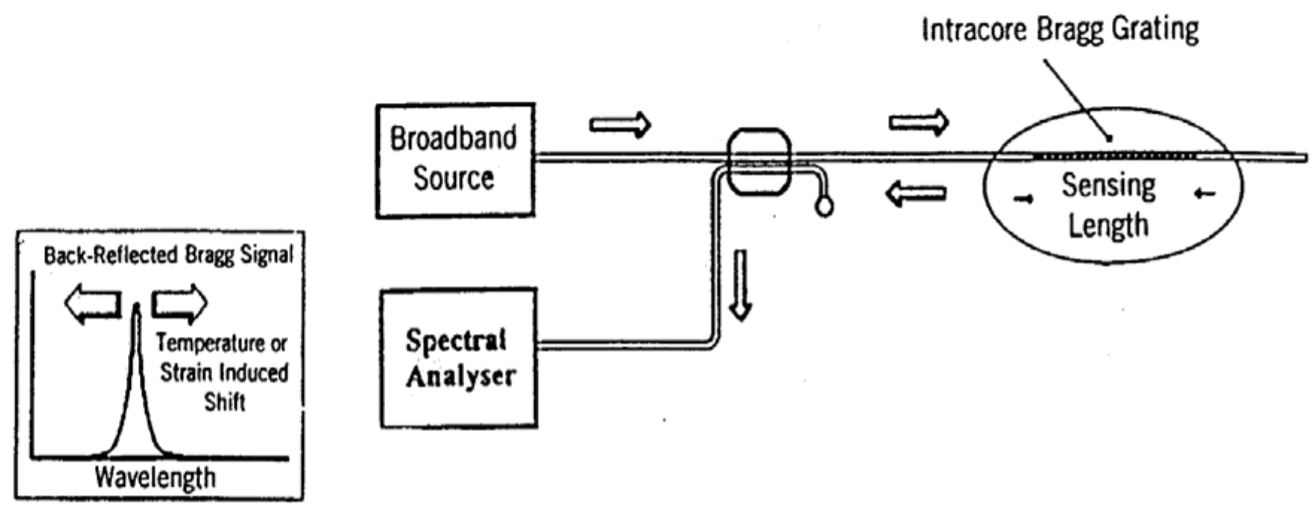
\includegraphics[width=0.85\textwidth]{./img/medicBragg}
			\caption{Representación esquemática de un sistema de  medición de deformaciones mediante fibras ópticas con redes de Bragg y analizador espectral óptico. \cite{tesisUPMmalte}} 
			\label{fig:medicBragg}
		\end{figure}
		
		Para utilizar las FBGs cómo sensores se puede construir una distribución como la de la figura \ref{fig:medicBragg}. En primer lugar, se manda un pulso a través de la fibra, y se pone un analizador de espectros para anotar las variaciones en la longitud de onda de Bragg ($\lambda\textsubscript{B}$). Según sea el escenario a sensar pueden ser necesarias más de una FBG. Para ello se puede realizar una configuración en serie (empalmando FBGs) o en paralelo (utilizando multiplexores). 
		
		\begin{figure}[H]
			\centering
			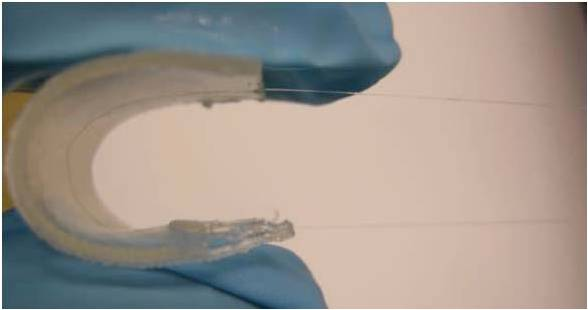
\includegraphics[width=0.65\textwidth]{./img/flexibleFBG}
			\caption{FBG embebida en un material flexible. \cite{nedomaPDMS}} 
			\label{fig:flexibleFBG}
		\end{figure}
	
		Además, para proteger la FBG es conveniente cubrirla con un material flexible (figura \ref{fig:flexibleFBG}), como por ejemplo el policloruro de vinilo (PVC) o el polidimetilsiloxano (PDMS). En este trabajo se utiliza como material protector y estructura del guante el PDMS, expuetso en el siguiente punto.
	
\end{itemize}


%-- POLIDIMETILSILOXANO - PDMS	
\subsection{Polidimetilsiloxano (\textit{PDMS})}
\label{sec:pdms3}
	
	Dentro de la familia de los polímeros orgánicos basados en silicio se encuentra el polidimetilsiloxano, también conocido como PDMS. Otro término por el que se le conoce es dimeticona, un tipo de aceite de silicona. Para abreviar, a partir de este punto en el documento se referirá a él como PDMS. El polidimetilsiloxano es un material cristalino, flexible y fácil de modelar \cite{propPDMS}.
	
	\begin{figure}[H]
		\centering
		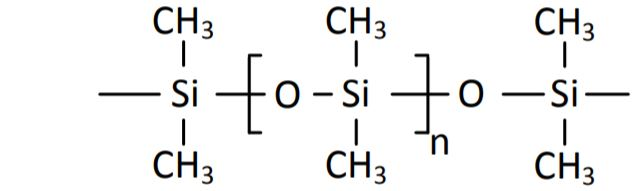
\includegraphics[width=0.45\textwidth]{./img/compPDMS}
		\caption{Composición química del PDMS. \cite{nedomaPDMS}} 
		\label{fig:compFBG}
	\end{figure}
	
	Su formulación química es $(H_{3}C)_{3}SiO[Si(CH_{3})_{2}O]_{n}Si(CH_{3})_{3}$ (figura \ref{fig:compFBG}), siendo $[Si(CH_{3})_{2}O]_{n}$ el monómero presente n veces en la molécula del PDMS según la proporción de este con el agente de curación \cite{propPDMS}.  	
 
 	Para su fabricación se mezcla el monómero con el agente de curación siguiendo una proporción n:1, en función de la consistencia con la que se desee el elastómero resultante. Cuanto mayor sea la n, mayor será la solidez del PDMS. Una vez hecha la mezcla es necesario que esta cure, ya sea a temperatura ambiente o aplicándole calor para que cure más rápidamente.
  
 	\begin{figure}[H]
	 	\centering
	 	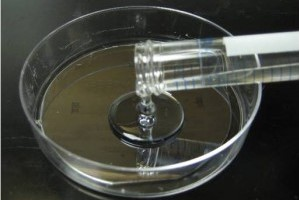
\includegraphics[width=0.49\textwidth]{./img/liquidoPDMS}
	 	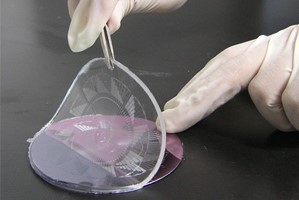
\includegraphics[width=0.49\textwidth]{./img/solidoPDMS} 
	 	\\(a)\hspace{7cm}(b)
	 	\caption{(a) PDMS en estado líquido \cite{liquidoPDMS} (b) PDMS en estado sólido, trás la curación \cite{solidoPDMS}} 
	 	\label{fig:slPDSM}
	 \end{figure}
  \textcolor{teal}{TENGO QUE ELEGIR ENTRE UNA PAREJA DE IMAGENES U OTRA, O UNA DE CADA. Debajo dejo los links de las de abajo por si necesito ponerlos en la bibliografia.\\}
  	\begin{figure}[H]
	 	\centering
	 	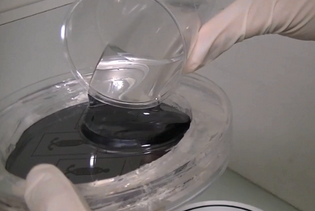
\includegraphics[width=0.49\textwidth]{./img/liquidPDMS}
	 	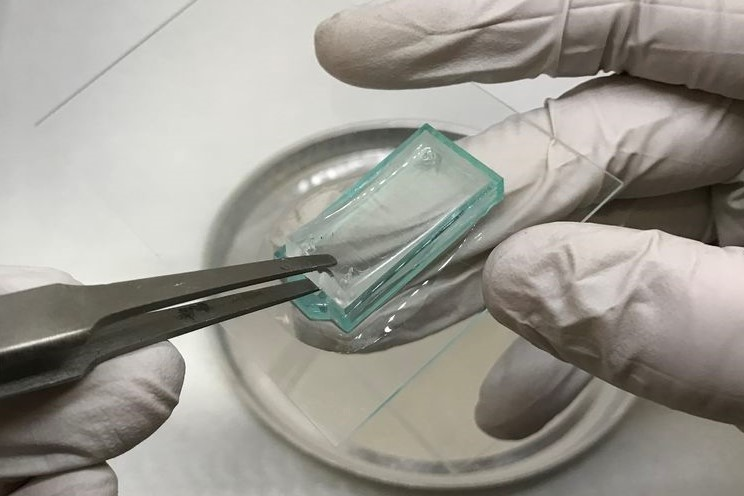
\includegraphics[width=0.49\textwidth]{./img/solidPDMS} 
	 	\\(a)\hspace{7cm}(b)
	 	\caption{(a) PDMS en estado líquido \cite{liquidoPDMS} (b) PDMS en estado sólido, trás la curación \cite{solidoPDMS}} 
	 	\label{fig:slPDSM2}
	 \end{figure}
 
 	\url{https://www.elveflow.com/microfluidic-tutorials/soft-lithography-reviews-and-tutorials/introduction-in-soft-lithography/pdms-softlithography-replication/}
 
	\url{https://www.instructables.com/id/Making-a-PDMS-Microfluidic-Device-With-Maskless-Mo/}
	
  	 La utilización de este elastómero en el ámbito de este trabajo es una buena opción ya que es inofensivo, no tóxico, no inflamable y eléctricamente no conductor.\cite{nedomaPDMS}

	% Material empleado para embeber las FBGs.


		
%-- LABVIEW 	
\subsection{LabVIEW (\textit{\underline{Lab}oratory \underline{V}irtual \underline{I}nstrument \underline{E}ngineering \underline{W}orkbech})}

\label{sec:labview3}



	\begin{figure}[H]
		\centering
		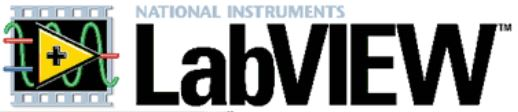
\includegraphics[width=0.45\textwidth]{./img/LabVIEWicon}
		\caption{Logo LabVIEW. }
		\label{fig:LabVIEWicon}
	\end{figure}

	LabVIEW es un software de National Instruments de ingeniería que pretende simplificar el diseño de sistemas software distribuidos de pruebas, medidas y control \cite{LabVIEWpage}. Es un lenguaje y un entorno de programación gráfica desarrollado por National Instruments. 
	
	En sus inicios LabVIEW estaba orientado únicamente a aplicaciones de control de equipos electrónicos utilizados para el desarrollo de sistemas de instrumentación. Tiene dos ventanas principales: el \textbf{Panel frontal} y el \textbf{Diagrama de bloques}, como se ve en la figura \ref{fig:ejLabVIEW}. El panel frontal alberga los botones, pantallas, etc. con el que el usuario interactúa una vez está desarrollado el software, interfaz de usuario. Mientras que el diagrama de bloques corresponde a la circuitería interna del programa, dónde se interconectan los elementos del panel frontal para operar con ellos, dando lugar a la programación del backend del software \cite{LabVIEWbook}. 
	
  	\begin{figure}[H]
		\centering
		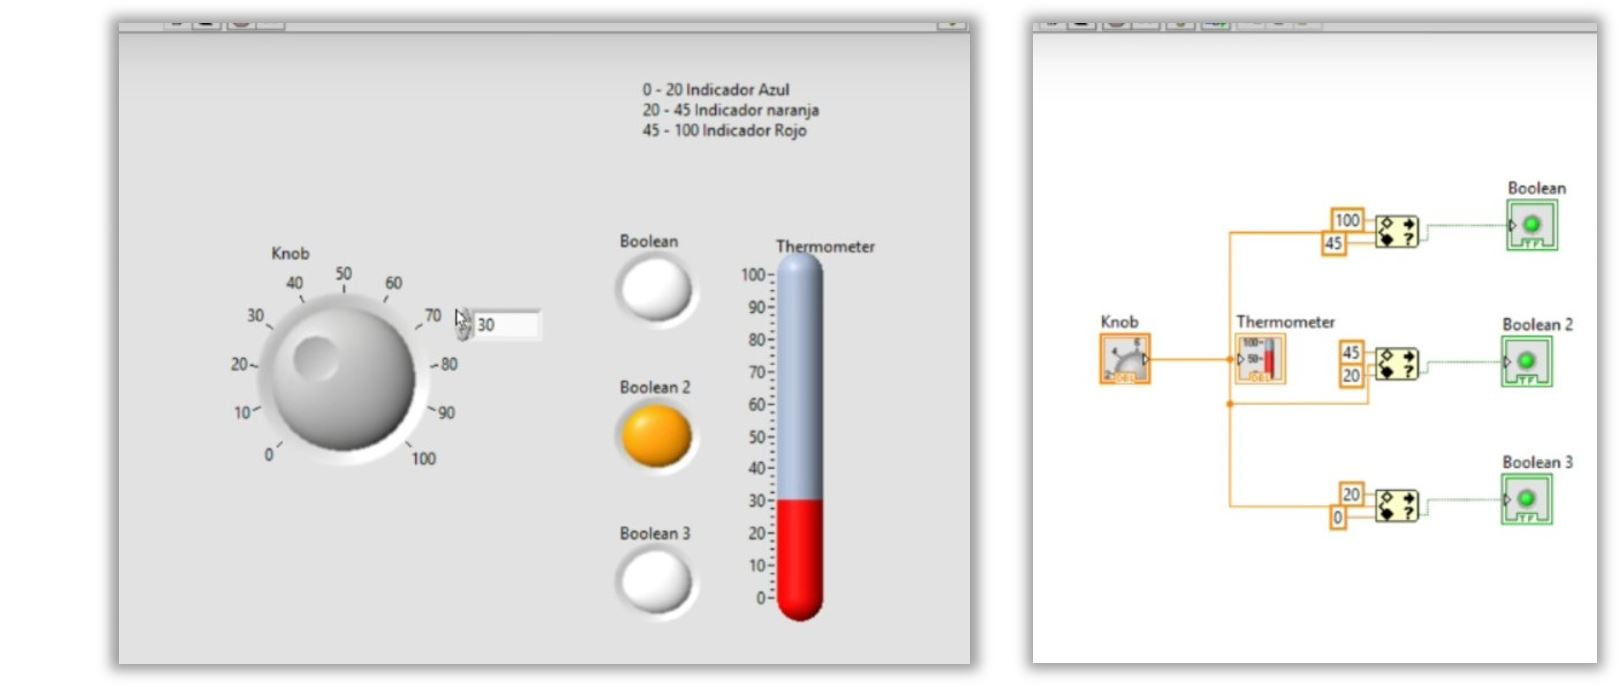
\includegraphics[width=0.95\textwidth]{./img/LabVIEWej}
		\\\hspace{2.5cm}(a)\hspace{6.5cm}(b)
		\caption{(Ejemplo sencillo de LabVIEW: (a) Frontend; (b) Backend}\cite{LabVIEWyt} 
		\label{fig:ejLabVIEW}
	\end{figure}

	En LabVIEW la programación se realiza en el Diagrama de bloques. Los programas están compuestos por los siguientes elementos: controles, funciones e indicadores. Estos elementos se conectan mediante "cables". De esta manera se genera el programa, definiendo la "circulación" de los datos.  
	

 \textcolor{rositaoscuro}{asdf}
 \textcolor{teal}{sdffsd}
%--Desarrollo del prototipo



\section{Desarrollo del prototipo}
\label{sec:prototipo3}
%[Esta parte de desarrollo del proyecto parte de otro trabajo. Aquí mencionar algo que diga el trabajo de Silvia y mencionar la en la bibliografía.]

La realización del primer desarrollo se origina a partir de un trabajo realizado con anterioridad en el grupo de investigación de la universidad\cite{SilviaTFM}. Se mejora el soporte físico(hardware) y se desarrolla un nuevo programa con un interfaz de usuario simple e intuitivo.

El prototipo consiste en un prototipo técnico y funcional de un guante, con sensores de FBG embebidos en PDMS. 
 
\subsection{Materiales}
\label{sec:materiales3}
En este apartado se disponen brevemente los componentes utilizados para el 
\begin{figure}[H]
	\centering
	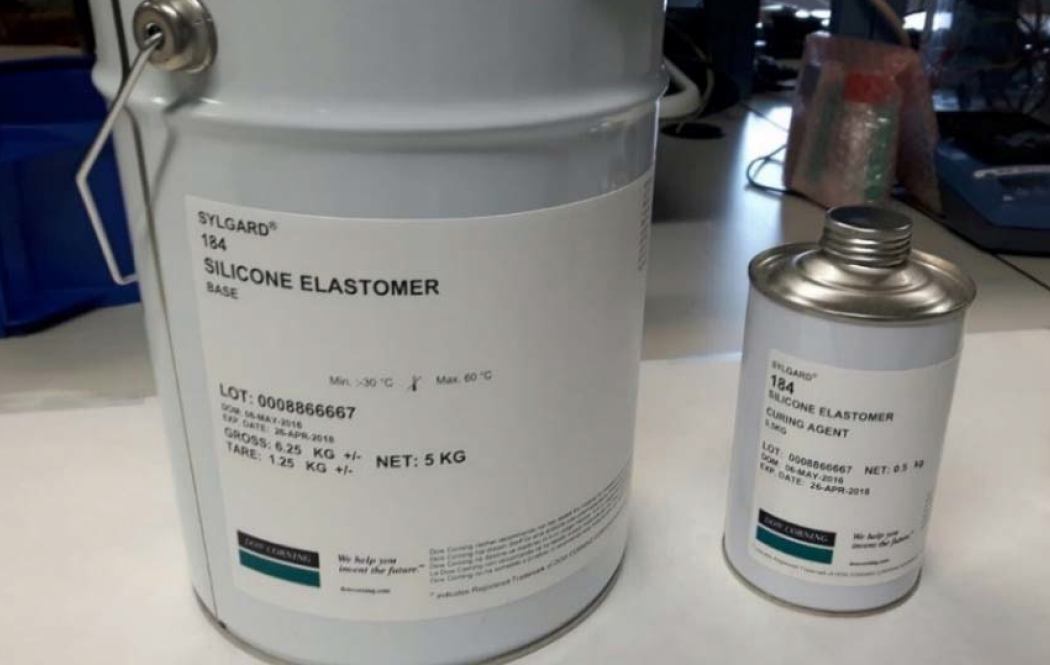
\includegraphics[width=0.75\textwidth]{./img/PDMS}
	\caption{PDMS: Elastómero y agente de cura.} \label{fig:pdms}
\end{figure}


\subsection{Proceso de fabricación del soporte físico}
\label{sec:proceso3}
%Elaboración
Para que sea más cómoda la explicación del proceso de elaboración del prototipo se divide este en tres partes: modelado 3D, fabricación del guante y montaje de prototipo completo.

\begin{itemize}
	\item \textbf{Modelado 3D - Configuración 3D}
	
	Esta actividad comprende el diseño del molde con el que se fabrica el guante y de la caja contenedora de todo el cableado.
	Para poder producir el guante de PDMS es necesario tener un molde donde verter la disolución para darle la forma deseada. Gracias a las versatilidad de diseño que ofrece la impresión 3D se realiza con este proceso de manufactura el molde (véase figura \ref{fig:molde}). 
\begin{figure}[H]
	\centering
	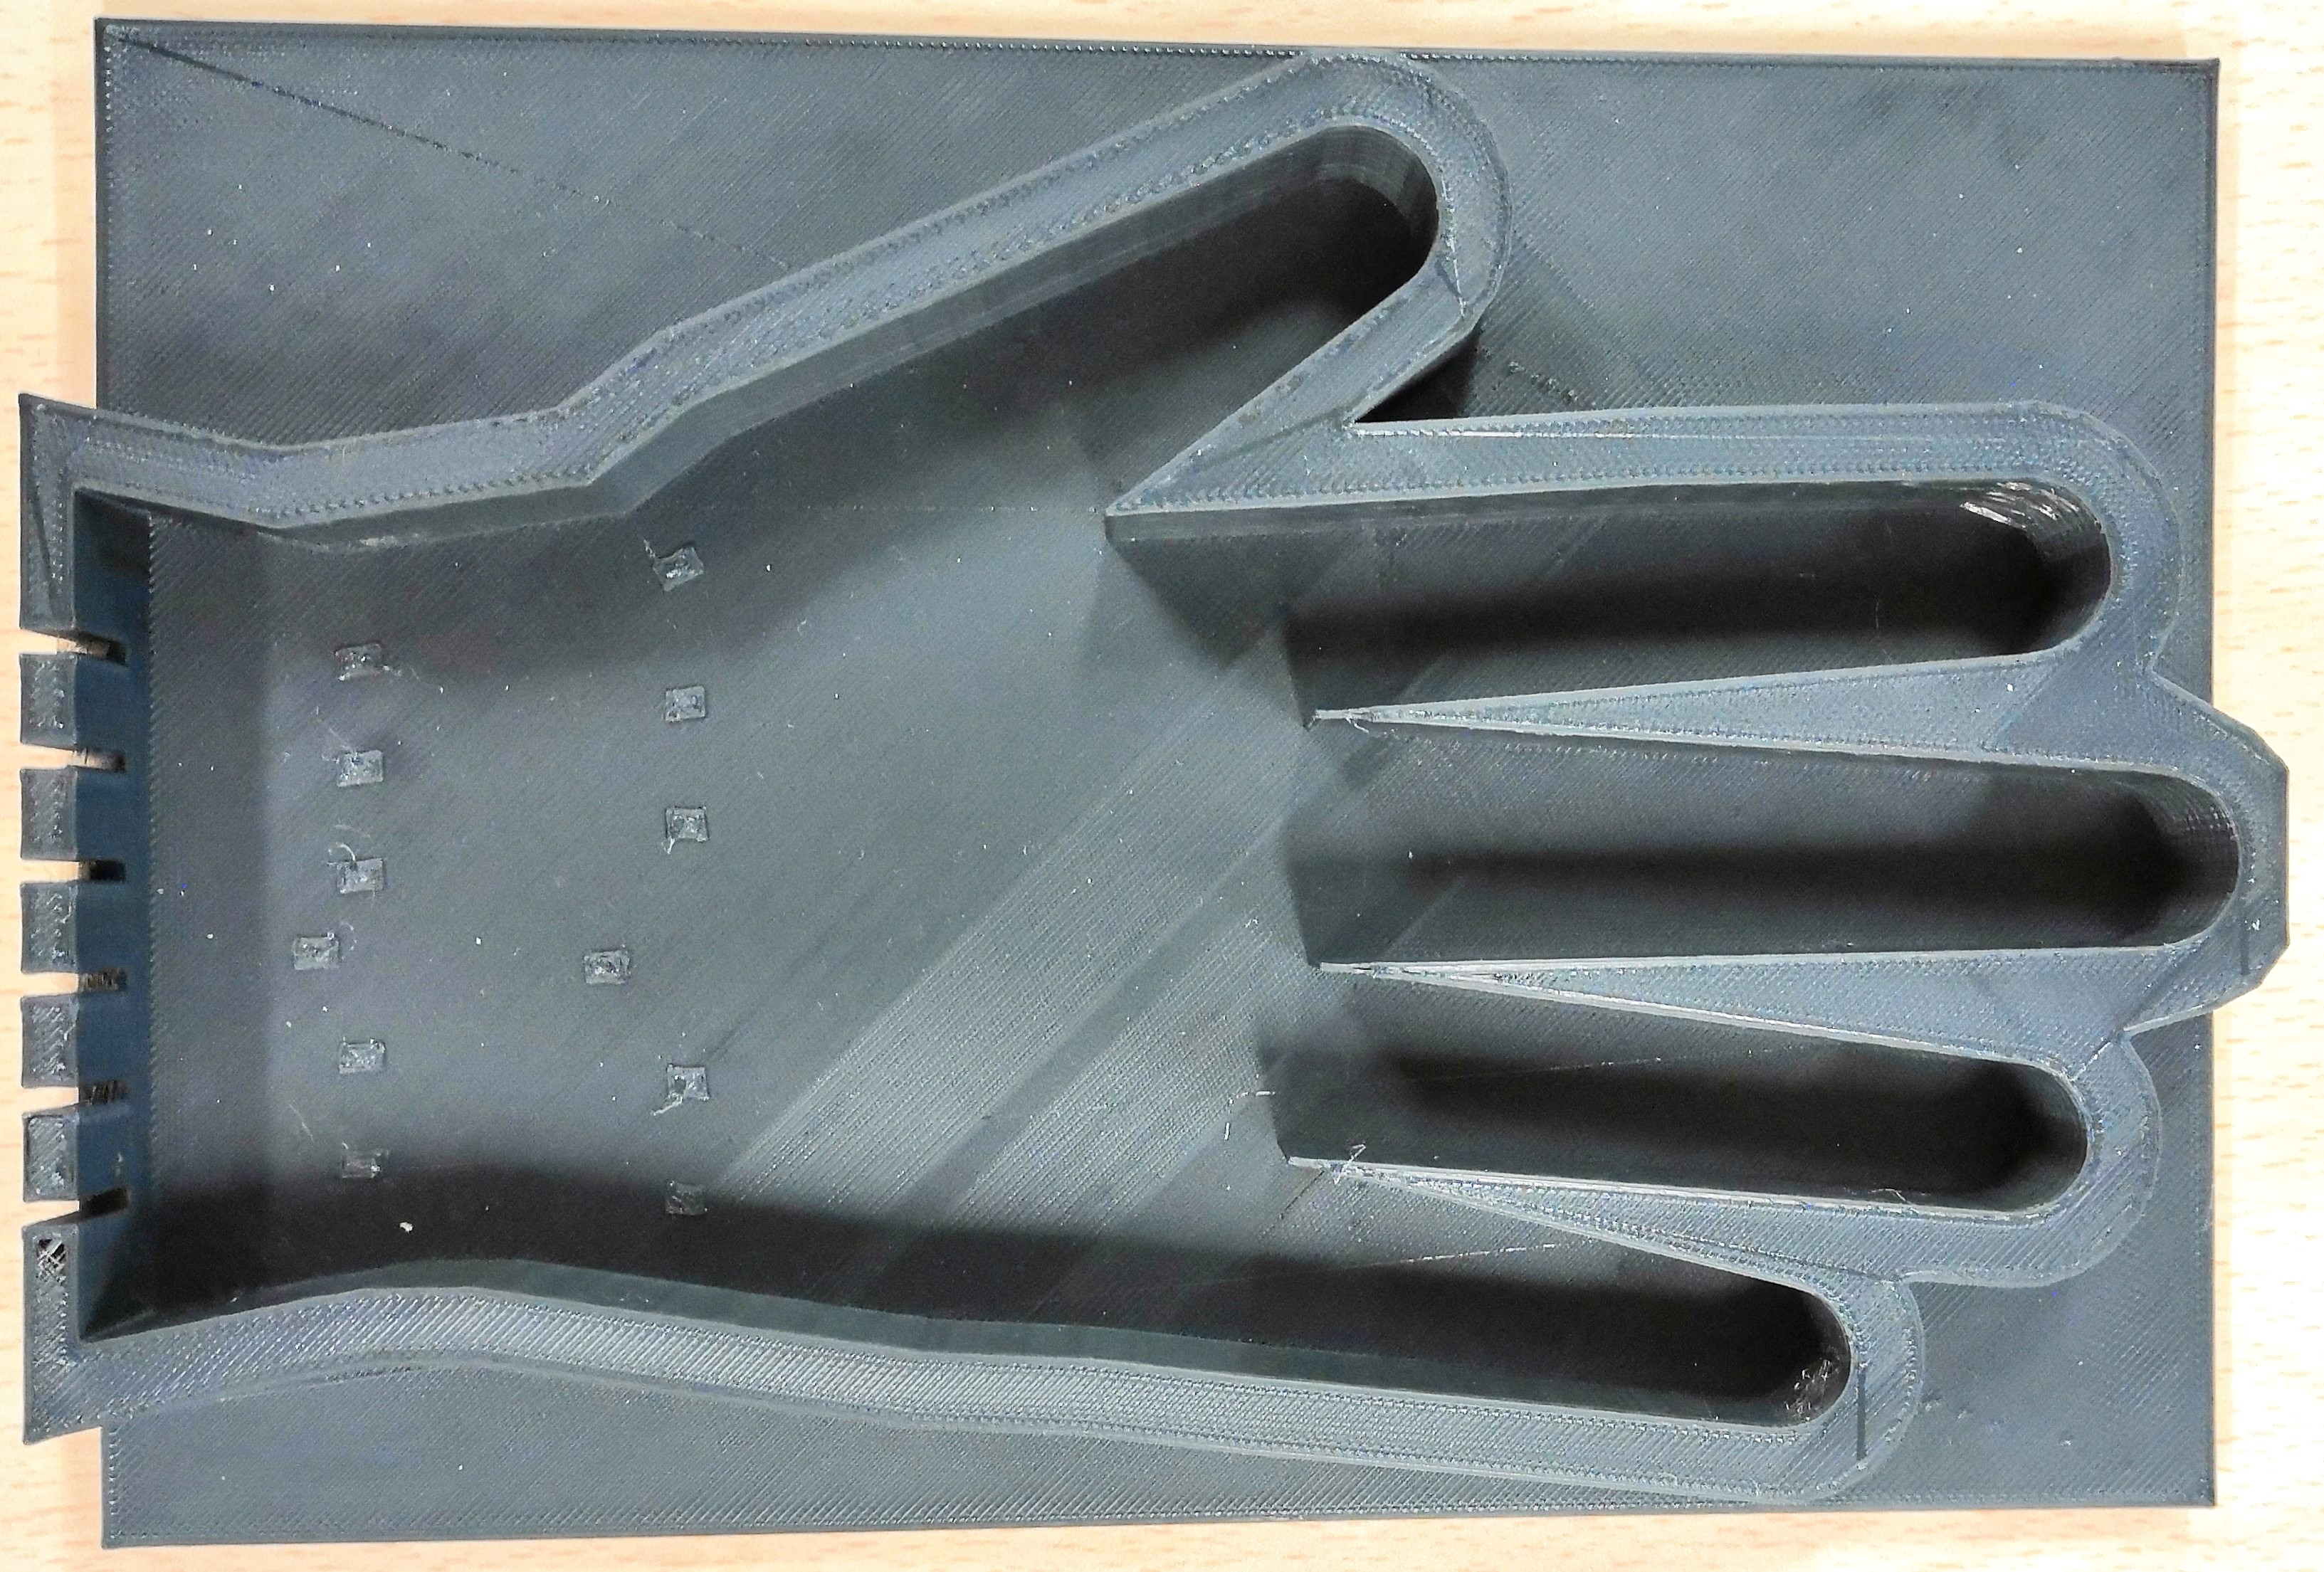
\includegraphics[width=0.5\textwidth]{./img/molde1}
	\caption{Molde} \label{fig:molde}
\end{figure}

	
 
	\item \textbf{Fabricación del guante}
	
	Para el proceso de fabricación del guante se necesitan ..................
	
	\begin{enumerate}
		\item Preparar mezcla PDMS (35g de polímero y 3.5g de agente de curación). Primero el
		elastómeto y después agente de curación.
		\item Revolver la mezcla durante al menos 4 minutos.
		\item Se deposita el PDMS y se colocan las fibras en el molde
		\item Se introduce en un horno de vacío para eliminar las burbujas durante 20 minutos, sin aplicar
		temperatura.
		\item Meter el molde en el horno (4h y media a $-55\,^{\circ}\mathrm{C}$). Dejar un poco más.
		\item Desmoldar.

	\end{enumerate}
	
	\textcolor{rositaoscuro}{Las siguientes figuras la puedo poner por separado, en la explicacin del procesado de emapalmar.}
	\begin{figure}[H]
		\centering
		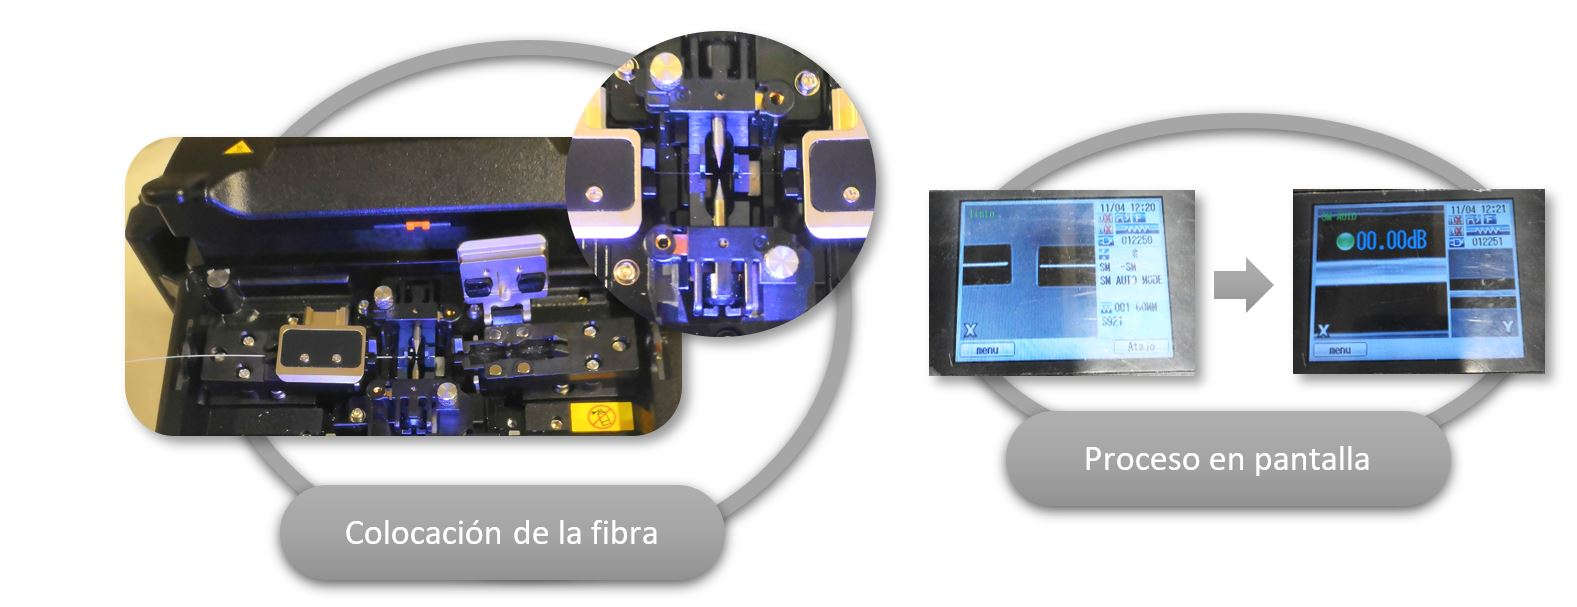
\includegraphics[width=0.95\textwidth]{./img/fusionFOpractica}
		\caption{Colocación de la fibra en la fusionadora y proceso por pantalla. \cite{FOAconect}} 
		\label{fig:fusionadora}
	\end{figure}  
	
	
	
	\item \textbf{Montaje completo}
	
	asdf
	
\end{itemize}

asdf


\begin{table}[H] %BORRAR
	\centering
	\begin{tabular}[t]{|c|}
		\hline
		\textbf{\textcolor{rositaoscuro}{BORRAR}} \\
		\hline
		longitudes de onda del guante de fibras cortas\\
		\hline
	\end{tabular}
	\begin{tabular}[t]{|r|c|}
		\hline
		 & Longitud de onda del sensor\\
		\hline
		\hline
		Dedo pulgar & 1512 nm \\
		\hline
		Dedo índice & 1520 nm \\
		\hline
		Dedo corazón & 1528 nm \\
		\hline
		Dedo anular & 1536 nm \\
		\hline
		Dedo meñique & 1544 nm \\
		\hline
		Muñeca & 1556 nm \\
		\hline
	\end{tabular}
	\caption{Tabla longitud de cada sensor FBG}
	\label{tabla:hmedidas 80 cm}
\end{table}
%-- Hasta aquí borrar la tabla.


\begin{table}[H]
	\centering
	\begin{tabular}[t]{|r|c|}
		\hline
		& Longitud de onda del sensor\\
		\hline
		\hline
		Dedo pulgar & 1532 nm \\
		\hline
		Dedo índice & 1548 nm \\
		\hline
		Dedo corazón & 1576 nm \\
		\hline
		Dedo anular & 1568 nm \\
		\hline
		Dedo meñique & 1560 nm \\
		\hline
		Muñeca & 1541.26 nm \\
		\hline
	\end{tabular}
	\caption{Tabla longitud de cada sensor FBG}
	\label{tabla:mmedidas 80 cm}
\end{table}

Para determinar la valid


\subsection{Funcionamiento}
\label{sec:funcionamiento3}
asdf

\begin{figure}[H]
	\centering
	\includegraphics[width=1\textwidth]{./img/interfazSM}
	\caption{Interfaz del programa de labview.}
	\label{fig:interfaz}
\end{figure}

%------IIIIIIMMMMMMUUUUUU------





\section{Resultados y análisis}
\label{sec:resultados3}

\section{Solución con sensores IMU}
\label{sec:IMU3}
asdf

\subsection{Marco conceptual}
\label{sec:mc3IMU}
asdf

\subsection{Desarrollo del prototipo}
\label{sec:prot3IMU}
asdf

\subsubsection{Materiales}
asdf


\subsubsection{Elaboración/Proceso de fabricación}
asdf

\subsubsection{Funcionamiento}
asdf




\section{---------------}

ME PLANTEO LA POSIBILIDAD DE DIVIDIR EL CAPITULO 3 EN CAPITULO 3 Y 4.


----------------------------------------------------------------------------------------------------------------------------------------------------------------------------------------------------------------------------------------------------------------------------------------------------------------------------------------------------------------------------------------------------------------------------------------------------------------------------------------------------------------------------------------------------------------------------------------------------------------------------------------------------------------------------------------------------------------------------------------------------------------------------------------------------------------------------------------------------------------------------------------------------------------------------------------------------------------------------------------------------------------------------------------------------------------------------------------------------------------------------------------------------------------------------------------------------------------------------------------------------------------------------------------------------------------------------------------------------------------------------------------------


\section{---------------}


\section{Sensores inerciales}
\subsection{Principio de funcionamiento}

Un sistema de referencia inercial se trata de un sistema de referencia regido por las leyes de movimiento de Newton. Por tanto, un sensor capaz de medir valores respecto a dicho sistema de referencia es lo que se conoce como un sensor inercial.

Una unidad inercial o IMU (Inertial Magnetic Unit) es un dispositivo que se compone de tres giróscopos (para determinar la orientación), tres acelerómetros y un reloj que permite asignar tiempo a los valores medidos por los sensores inerciales. Dichas unidades inerciales presentan tres ejes y cada uno de ellos presenta un acelerómetro y un giróscopo.

Por tanto, la información que se recoge de las unidades inerciales son aceleraciones lineales, velocidades angulares y tiempo común para los tres ejes que llevan dicha información de aceleración y velocidad angular (ver Figura \ref{fig:Imu}). 


El tiempo requerido para la implementación del sistema de medida puede influir en la marcha de los pacientes y por tanto en la obtención de los parámetros \cite{begona}. Los sensores inerciales utilizados permiten realizar las mediciones de una manera sencilla y rápida lo cual resulta beneficioso en el contexto ambulatorio tanto para los pacientes como para el personal sanitario



\subsection{Sensores inerciales propuestos}
Los sensores inerciales utilizados para el sistema son el modelo MTw Awinda (Xsens Technologies B.V, The Netherlands) pueden verse representados en la Figura \ref{fig:sensor_XSENS}



Su tamaño es de 47 x 30 x 13mm y 16g de peso por lo que puede definirse como un sistema compacto y ergonómico que será de utilidad para el sistema propuesto en este trabajo. Dispone de unas bandas de sujeción que permiten colocar el sensor en el lugar necesario y por tanto dota de versatilidad al diseño. 

Además, se incluye un software de captura que resultará útil para obtener las señales para su posterior procesado. La comunicación de los sensores con el software emplea un protocolo propietario que aparece representado en la Figura \ref{fig:protocolo}.

\subsubsection{Sensores inerciales}

	
	Para la obtención del dato de distancia a partir de las señales proporcionados por los sensores inerciales es necesario tener en cuenta que la distancia se recorre en el plano en el que se produce el avance, que es este caso es el plano XY.

Para obtener la posición en este plano a partir de la aceleración en los tres ejes XYZ proporcionada por los sensores inerciales, es necesaria una doble integración.Posteriormente se elimina la deriva existente en las señales debido a esta integración. A continuación se describen los cálculos realizados

Una vez calculadas las distancias necesarias, se procede al cálculo de la distancia de separación entre pasos. En la Figura \ref{fig:sep} se representa dicho cálculo. La distancia D2 es la correspondiente al cálculo de la distancia con el sensor inercial izquierdo en este caso, la distancia D1 es la distancia calculada mediante el sensor de ultrasonido.
\begin{figure}[H]
	\centering
	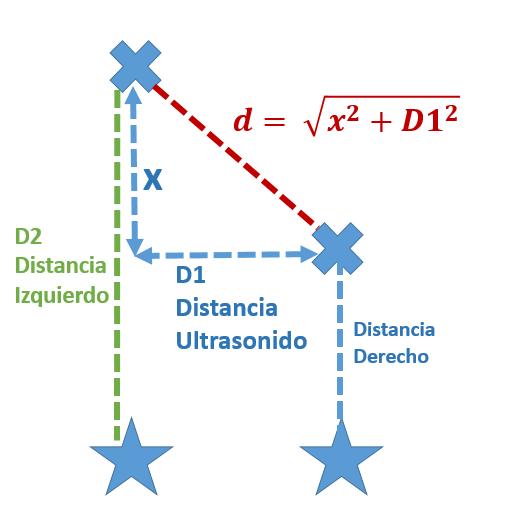
\includegraphics[width=0.8\textwidth]{./graphics/sep}
	\caption{Cálculo final de distancia de separación entre pasos} \label{fig:sep}
\end{figure}

Por tanto, para obtener X se utiliza la ecuación \ref{eq:x}
\begin{equation}\label{eq:x}
x = D2 - DistanciaDerecho
\end{equation}
En el caso de que el primero de los pasos se comenzase con el izquierdo la ecuación es la relativa a la DistanciaIzquierdo.

Para determinar la distancia, se utiliza por tanto, la ecuación \ref{eq:d}
\begin{equation}\label{eq:d}
d = \sqrt{x^{2}+D1^{2}}
\end{equation}